\chapter{Introduction a EMMA}
\label{ch:introduction}
% (cf loi de \cite{moore1965cramming}). 
%\cite{THOMPSON200620}

%Les échelles de temps sont radicalement opposées entre la cosmologie qui considère les temps les plus long de l'univers et les progrès informatiques qui vont à une vitesse exponentielle.
%Du fait de l'avancée rapide des moyens de calculs, les simulations numérique sont des produits possédant une valeur se dépréciant rapidement et doivent être considérées comme éphémère.

Nous avons vu dans la partie précédente qu'elles étaient les principales physiques à l’œuvre durant l'époque de réionisation.
L'objectif de cette partie est d'expliquer comment ces physiques sont modélisées et quelles sont les contraintes sur leurs implémentations.
On se concentrera particulièrement sur le cas du code EMMA.


%Comment modéliser la reionization?

\section{Aperçu des différents modèles numériques}

Un code de simulation cosmologique a pour vocation principale de suivre l'évolution de différents "fluides", comme la matière noire, la gaz, les étoiles et la radiation (et parfois le champs magnétique).
Ces fluides sont de natures différentes et il n'y a pas de méthode unique permettant de suivre de manière optimale ces différentes physiques.
On distinguera principalement deux catégories de fluides: les collisionnels et les non-collisionnels.
La physique non-collisionnelle concerne les phénomènes qui n'interagissent pas par collision comme la matière noire, les étoiles ou la radiation. 
La physique collisionnelle concerne qant à elle principalement l'hydrodynamique du gaz.

Il existe conceptuellement deux principales façons de suivre un fluide dans l'espace.
%Ces deux approches sont dites \emph{Eulérienne} ou \emph{Lagrangienne}.
%En lien direct avec ces deux familles de représentations physique, il existe deux principales familles de codes cosmologique% : les codes \ac{SPH} et les codes \ac{AMR}.

\paragraph{Représentation Lagrangienne : } 
consiste à se placer au point de vue du fluide.
Une série d'éléments de fluide de masse fixe pouvant se déplacer et/ou se dilater dans l'espace sera considérée.
Les codes utilisant ce type de représentation seront généralement associés avec une gestion de la physique sous forme de \emph{particules}.
Ces codes seront dit \ac{SPH} ou \ac{PIC}.

%\paragraph{\ac{SPH} : } représente le gaz sous forme de particule de masse constante mais de taille variable.
%Notion d'arbre -> KDtree

\paragraph{Représentation Eulérienne : } 
consiste à se placer au point de vue de l'espace.
On considère un élément d'espace et le bilan de matière entrant et sortant de chacune de ses interfaces.
On associera généralement les codes utilisant ce type de représentation avec une gestion de la physique sous forme de \emph{grille}.
Si la grille est de résolution variable, on parlera de grille \ac{AMR}.

%\paragraph{Code sur grille} : représente l'espace sous forme de cellules organisées sur une grille. 
%Notion d'arbre -> arbre AMR
%La représentation Lagrangienne la plus populaire (dans le domaine des simulations cosmologiques) est sans doute le \emph{Smouth Particle Hydrodynamics (SPH) }
%Les volumes cosmologiques étant généralement cubique, les éléments de grille le sont généralement aussi.
%historique
%avantage inconvénient AMR vs SPH
%introduction de la grille et de la méthode AMR

Un même code peux utiliser conjointement plusieurs des concepts qui viennent d'être introduits.
Dans le cas présent, EMMA utilise une représentation Lagrangienne pour simuler la physique non collisionnelle de la matière noire et des étoiles, et une représentation Eulérienne pour simuler le gaz et la radiation.

\subsection{Quelques codes de simulations cosmologiques}

Il existe une certaine variété de code de simulations cosmologiques.
Ces codes sont classés en fonction de leur façon de gérer l'hydrodynamique du gaz et on distinguera principalement les codes \ac{SPH} et les codes \ac{AMR}.

Parmi les représentants des codes \ac{SPH} :
\begin{itemize}
\item GADGET \citep{springel_cosmological_2005}
\item GASOLINE2 \citep{2017arXiv170703824W}
\item PHANTOM \citep{2017arXiv170203930P}
\end{itemize}

Parmi les représentants des codes \ac{AMR}:
\begin{itemize}
\item ART \citep{1997ApJS..111...73K}
\item FLASH \citep{0067-0049-131-1-273}
\item RAMSES \citep{teyssier_cosmological_2002}
\item ENZO \citep{bryan_enzo:_2014}
\item EMMA \citep{aubert_emma:_2015}
\end{itemize}

Il existe un troisième type de code hybride utilisant une maille mobile et adaptative, un représentant majeur de cette technique est le code AREPO \citep{2010MNRAS.401..791S}.

%\subsection{AMR et SPH}

Des projets comme le projet Santa Barbara \citep{1999ApJ...525..554F} ou le projet nIFTy \citep{sembolini_nifty_2015} visent à comparer les codes de différents types entre eux.
Certain projets \citep{2007MNRAS.380..963A, oshea_comparing_2005} se focalisent sur la comparaison des méthodes.
Il en ressort que l'\ac{AMR} est plus apte à gérer les chocs et les instabilités de type Kelvin–Helmholtz ou Rayleigh–Taylor.

%avantage inconvénient AMR vs SPH?


\subsection{RAMSES}

EMMA est largement inspiré de RAMSES \citep{teyssier_cosmological_2002}.
Ce dernier est une référence reconnue dans le domaine  des simulations cosmologiques et utilise des principes éprouvés, et EMMA en utilise un bon nombre.
Entre autre, la gestion de la grille le moteur hydrodynamique et le moteur radiatif sont similaires.
Le développement d'EMMA vise à obtenir une expertise complète sur le fonctionnement de ce type de code.

EMMA a cependant quelques différences fondamentale avec RAMSES.
Il n'utilise pas le même langage: RAMSES est écrit en Fortran, EMMA en c.
Le développement de RAMSES a débuté avant l'apparition des \ac{GPU} et a ensuite été adapté pour en utiliser les capacités de calcul.
EMMA est développé avec cette idée dès le départ, ce qui permet l'utilisation de certaines techniques menant à une implémentation différente.


\section{Gestion de la grille}
\label{sec_gestion_grille}
%(nécessaire d'être positionné ici car la structure en arbre conditionne plusieur choix par la suite)

Un des concepts central de EMMA est sa grille adaptative.
Tout les moteurs physiques sont basés dessus et sa structure conditionne un certain nombre de choix par la suite.
C'est pourquoi nous allons la développer ici, avant de détailler la gestion de la physique. 

\subsection{Grille régulière et AMR}
Avant d'aborder le concept de grille adaptative faisons un léger détour par l'exemple d'une grille fixe et régulière.
Dans le cas des simulations sur grille fixe, les données sont réparties en mémoire de façon ordonnée.
Dans un espace en 3D, on accédera à une cellule contenant le point de coordonnées normées $(x,y,z)$ sur une grille de $N_x*N_y*N_z$ cellules, à l'aide de son identifiant Id dans le tableau en mémoire.
\begin{equation}
Id = i + j*N_x + k * N_x*N_y
\end{equation}
avec :
\begin{equation}
\begin{cases}
i=\lfloor x \rfloor \cdot N_x \\
j=\lfloor y \rfloor \cdot N_y \\
k=\lfloor z \rfloor \cdot N_z \\
\end{cases}
\end{equation}
ou $\lfloor a \rfloor$ représente la partie entière de $a$.

Nous voyons ici que l'organisation en mémoire et la recherche de voisin sont relativement simple à gérer.
Les vecteurs sont alloués de manière statique et la recherche de voisin est basée sur un jeu d'indice relativement simple.
Les choses sont plus complexes dans le cas d'une grille adaptative.
Étant amenée à évoluer, il faut introduire des mécanismes permettant de construire ou détruire certaines parties de la grille de façons dynamique.
Ces mécanismes vont totalement changer l'organisation de la grille.

Un exemple de grille \ac{AMR} générée par EMMA est présenté sur la figure \ref{fig:AMR}).
Un fonction de critères prédéfinis par l'utilisateur la résolution de la grille peut être arbitrairement augmentée localement.
L'avantage de ce type de grille est d'économiser des ressources de calcul par rapport au cas d'une grille fixe, ou il faudrait beaucoup plus de cellules pour obtenir une résolution équivalente.

\begin{figure}[bth]
        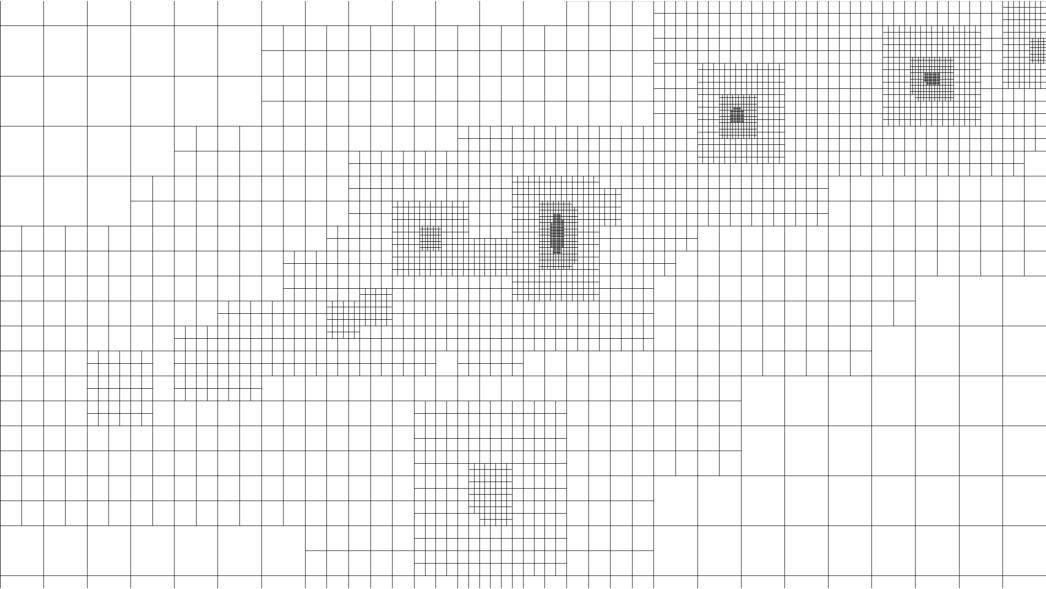
\includegraphics[width=.95\linewidth]{img/02/AMR.pdf} 
        \caption[Grille générée par EMMA]{Exemple de grille \ac{AMR} générée par EMMA. 
        La  résolution de la grille est augmentée arbitrairement dans les régions d'intérêts.
 		\label{fig:AMR}}
\end{figure}

\subsection{Octree}

Il existe deux grands groupe de maille adaptative.
Le premier groupe utilise une séries de grilles fixes imbriquées (eg \cite{bryan_enzo:_2014}) %TODO ref
Chaque région raffinée sera une grille fixe de résolution plus importante spatialement liée a une grille de base.
Chaque nouvelle grille aura une résolution double par rapport a la précédente.
Il est possible d'ajouter autant de niveaux que voulu.

EMMA utilise un second groupe. % fully threated tree description .
La base de cette représentation est de considérer que chaque cellule est associée à une grille fixe de taille 2x2x2 que l'on nommera un OCT, car décomposé en 8 cellules \citep{khokhlov_fully_1998-1}.
%sous parties qui sont elles même des cellules.
Et récursivement, chacune de ces cellules peuvent à leurs tour être divisée et associée à un OCT.
Il en résultera un arbre nommé Octree, représenté sur la figure \ref{fig:octree}.

\begin{figure}[bth]
        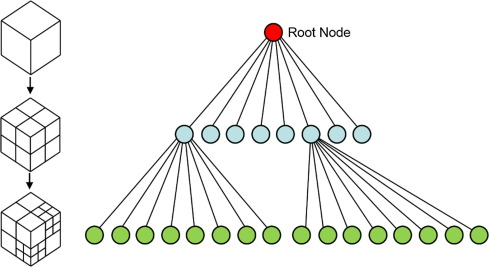
\includegraphics[width=.95\linewidth]{img/02/octree.jpg} 
        \caption[Grille AMR et son octree]{Représentation d'une grille AMR a gauche, et de son octree associé a droite. 
        Image extraite de \cite{SU201659}
     	\label{fig:octree}
}
\end{figure}

Pour créer une grille de départ, il faudra d'abord créer un OCT, appelé racine, et le forcer à raffiner.
Chacune de ces nouvelles cellules vont à leurs tours être raffinée.
Cette opération est répétée pour toutes les cellule jusqu'à obtention d'une grille régulière de la taille désirée.
A chaque nouveau raffinement le nombre de cellule est multiplié par 8.
Le nombre de cellules d'un niveau entièrement raffiné est donc de:
\begin{equation}
N_{cells} = 2^{3L}
\end{equation}
où $L$ est le niveau de raffinement.

Il en résultera une grille régulière qui ne pourra pas être dé-raffinée par la suite.
Le niveau de cette grille de base sera appelé niveau \textit{coarse}.

\subsubsection{La structure OCT}
%et liste chainée

Il existe une bimodalité entre la représentation de la grille en mémoire et la représentation de l'espace physique.
Comme la grille est amenée à évoluer, il n'y a plus une position unique en mémoire associée à une position dans l'espace.
De plus, le nombre d'éléments de la grille change au cours du temps.
Il faut donc conserver à la fois l'information de la position dans l'espace physique et dans l'espace mémoire.

En principe, on allouera une certaine quantité d'OCT en mémoire qui constituerons une réserve.
On viendra ensuite piocher dans cette réserve pour ajouter des éléments à la grille.
Les OCT de la grille seront organisés sous forme de liste chainées, il est donc nécessaire d'avoir l'information de la position de l'OCT précédent et de l'OCT suivant en mémoire.

Pour créer un lien entre elle, il est nécessaire de stocker l'information de voisinage.
L'information spatiale est aussi contenue dans les OCT, ceux ci disposent de six pointeurs vers les cellules voisine.
Un OCT est également composé d'un tableau de huit cellules filles, ainsi que d'un pointeur vers sa cellule mère.
Un OCT qui n'a pas de cellule mère est appelé OCT racine, en pratique il n'y en a qu'un seul, de niveau 0, et il représente l'ensemble de l'espace de la grille..
La génération de conditions périodique (généralement utilisées en cosmologies) se fait de manière naturelle en faisant pointer tout les voisins de l'OCT racine vers lui même.
La structure minimal d'un OCT de EMMA est présenté sur le listing \ref{lst:oct}.

\begin{lstlisting}[float=bth,language=C,frame=tb,caption={La structure OCT de EMMA},label=lst:oct]
struct OCT{
  struct CELL cell[8]; // les 8 cellules de l'oct
  struct CELL *nei[6]; // pointeurs sur les cellule voisines
  struct CELL *parent; // cellule mere
  struct OCT *next;    // oct suivant dans la liste chainee
  struct OCT *prev;    // oct precedent dans la liste chainee
  int level;           // niveau de l'oct
};
\end{lstlisting}

\subsubsection{La structure CELL}
\label{sec:CELL}
Les cellules contiennent l'information physique (densité, pression, température, etc...).
Chaque cellule peut, sous certaine condition, être subdivisée en un OCT pour augmenter la résolution localement.
L'information de la position de la cellule dans l'OCT parent est contenue dans son identifiant (allant de 0 à 7).
Une CELL qui n'a pas d'OCT enfant est dite cellule feuille.
La structure minimal d'une CELL de EMMA est présenté sur le listing \ref{lst:cell}.

\begin{lstlisting}[float=bth,language=C,frame=tb,caption={La structure CELL de EMMA},label=lst:cell]
struct CELL{
  int id;            // permet de determiner la position de la cellule dans l'oct
  struct OCT *parent // l'oct pere de la cellule
  struct OCT *child; // si child est different de NULL alors la cellule est raffinee et child point vers l'oct enfant
  struct PHYSIC *data; // pointeur vers la partie physique
  struct PARTICLE *part; // pointeur vers la chaine de particules.
};
\end{lstlisting}


\subsubsection{La structure PARTICULE}
\label{sec:PART}

%TODO introduire liste chainée de particule

Nous verrons dans la section \ref{sec:solverDM} qu'une partie de la physique est résolue sous forme de particule.
Il est donc nécessaire d'ajouter un champs de particule à la grille \ac{AMR}
Comme les OCT, les particules utilisent une représentation sous forme de liste chaînée, et chaque cellule dispose de sa propre liste chaînée de particules.
Lors de raffinement cette liste devra être découpée et distribuée entre les nouvelles cellules crées.
Une particule est essentiellement caractérisée par sa position, sa masse et sa vitesse.
On ajoutera a ceci son statut, qui sera utilisé pour différentier les particules de matière noire des particules stellaires. 
Le listing \ref{lst:part} présente la structure minimale d'une particule dans EMMA.


\begin{lstlisting}[float=bth,language=C,frame=tb,caption={La structure PARTICULE de EMMA},label=lst:part]
struct PART{
  REAL3 x;  // vecteur position
  REAL3 v;  // vecteur vitesse
  struct PARTICULE *next;  // particule suivante
  struct PARTICULE *prev;  // particule precedente
  int idx;  // identifiant unique
  int  isStar;  // matiere noire ou etat de l'etoile
  REAL t;       // instant de creation
  REAL mass;    // masse
};
\end{lstlisting}



%TODO introduire la structure part

\subsection{Gestion du raffinement}
\label{sec:raffinement}
%différentes condition de raffinement.\\
%sur la matière noire\\
%semi Lagrangienne\\
%sur le gradient d'ionization\\
%sur le gradient de densité (shock)\\
\subsubsection{Condition de raffinement}
Il est possible de définir arbitrairement une condition de raffinement en fonction de la physique que l'on cherche a étudier.
Par exemple, dans des tests unitaires de type sphère de Stömgren (cf \ref{sec:stromgren}) ou explosion de Sedov (cf \ref{sec:sedov}), on marquera les cellules qui sont soumises à un gradient d'ionisation ou de densité supérieur à un certain seuil pour suivre l'évolution du front.
Dans le cas de simulations cosmologique, on utilisera généralement une condition en densité dite semi-Lagrangienne.
C'est a dire qu'une cellule sera marquée comme "à raffiner" si la masse de matière noire (ou de gaz) qu'elle contient est supérieur à huit fois la masse de matière noire (ou de gaz) moyenne d'une cellule de ce niveau.
%le deraffinement
On remarquera que la condition de raffinement ne prends pas en compte le fait qu'une cellule soit déjà raffinée ou non.
Si une cellule est raffinée, mais qu'elle n'est pas marquée comme "à raffiner" elle sera donc dé-raffinée.

\subsubsection{En pratique}
Le raffinement se fera en trois temps:

\begin{itemize}
\item Dans un premier temps le code va passer en revue toutes les cellules d'un niveau, et les marquer comme "à raffiner" si une première condition physique est respectée.

\item Une fois tout le niveau passé en revue, le code va ensuite faire une série de $N_{buffer}$ passages sur tout le niveau en marquant à chaque fois toues les cellules voisine des cellules précédemment marquées.
Cette zone de $N_{buffer}$ cellules autour des zones soumises à la condition physique de raffinement sera appelée le "buffer de raffinement".
Ce tampon a pour but d’élargir la zone de raffinement et ainsi permettre une transition douce entre les niveaux.
De plus il ne sera autorisé à n'avoir qu'un seul niveau de décalage au maximum lors des transitions.

\item Une fois les cellules respectant ces deux conditions marquées, le raffinement est effectué.
\end{itemize}

%En pratique le raffinement d'une cellule se fera en lui associant un OCT.
%*child pointera alors vers le dernier OCT libre de la liste chaînée.


\subsubsection{Opérateurs de changement de grilles} 
\label{Opérateurs de changement de grilles}

Les opérations de raffinement/dé-raffinement font intervenir des opérateurs de changement de grille.
Le changement de résolution peut avoir lieu dans les deux sens :

\begin{itemize}
\item La \emph{restriction} consiste à dégrader la grille en résolution. 
La restriction la plus directe consiste à moyenner les cellules à dégrader. 
Par exemple, sur une grille à deux dimensions, pour diviser la résolution par deux, quatre cellules de la grille de départ devront être moyennées pour obtenir une nouvelle cellule de la grille à base résolution.

\item La \emph{prolongation} consiste à augmenter la résolution d'une grille, la prolongation la plus directe consiste à injecter les valeurs de l'ancienne grille dans un certain nombre de cellules de la nouvelle grille. (fig \ref{Opérateurs de changement de grille})
\end{itemize}

\begin{figure}
\begin{center}
\subfloat[Restriction]{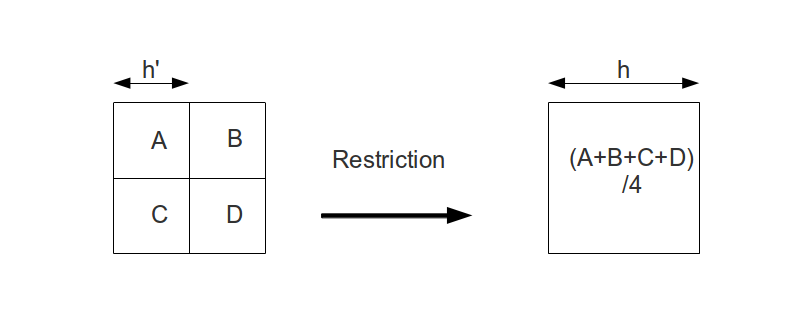
\includegraphics[width=.45\linewidth]{img/02/Restriction.png}}
\subfloat[Prolongation]{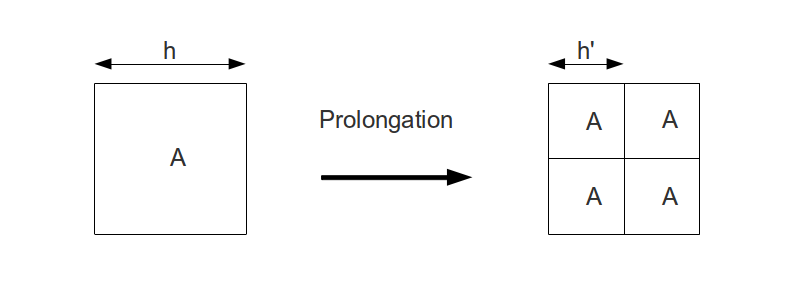
\includegraphics[width=.45\linewidth]{img/02/Prolongation.png}}\\
\subfloat[Niveau L  ]{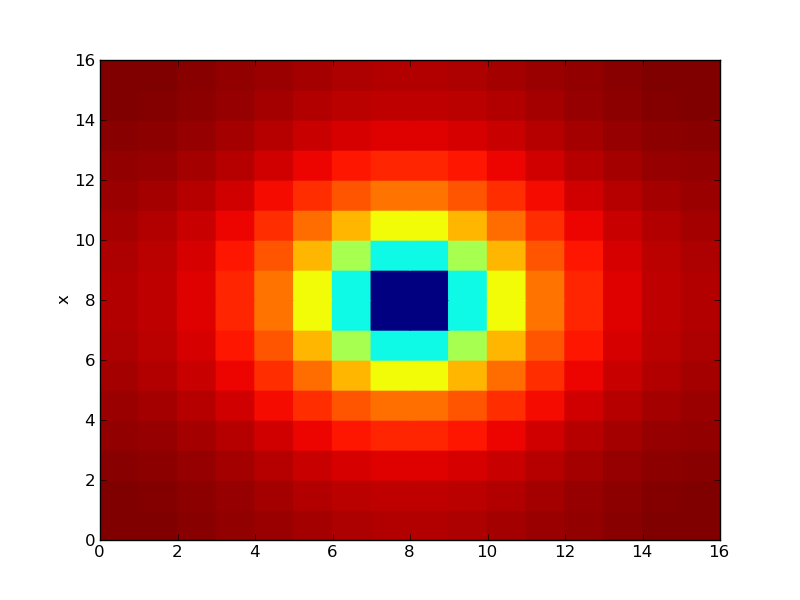
\includegraphics[width=.45\linewidth]{img/02/0090.png} \label{Opérateurs de changement de grille d}}
\subfloat[Niveau L+1]{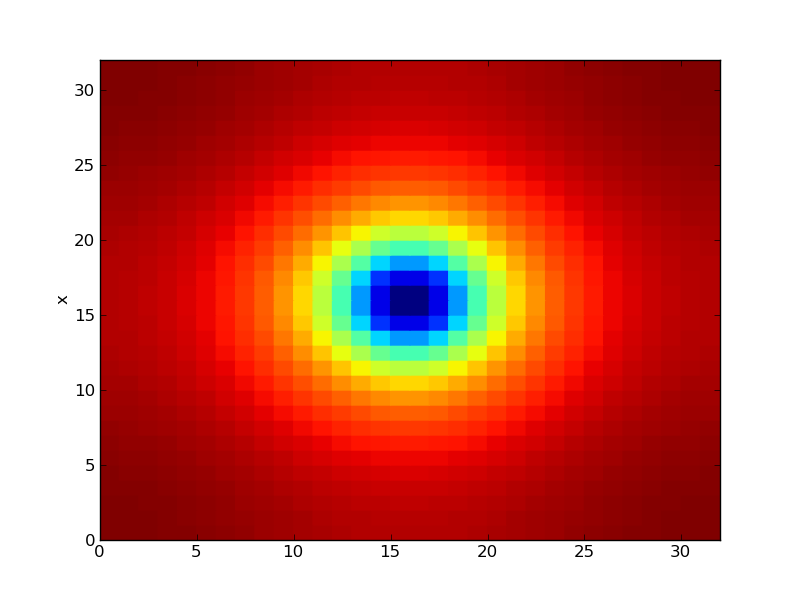
\includegraphics[width=.45\linewidth]{img/02/0088.png} \label{Opérateurs de changement de grille c}}
\caption[Opérateurs de changement de grille]{Opérateurs de changement de grille. 
Ils permettent de changer la résolution de la grille. 
Un exemple de restriction consiste à moyenner une valeur de plusieurs cellules, la prolongation associée consiste en une injection directe d'une valeur dans plusieurs cellules.
\label{Opérateurs de changement de grille}}
\end{center}
\end{figure}

%La prolongation et la restriction sont des opérateurs aisément parallélisables. Chaque cellule (ou paquet de huit cellules) est indépendante des autres et il est possible de ne changer la résolution que d'une partie de la grille sans en affecter le reste.

%Il existe principalement deux conditions sur les opérateurs de changement de grille. 
%La première impose une certaine réciprocité entre eux, les opérateurs doivent être adjoints: il est nécessaire qu'après une prolongation, suivie d'une restriction la grille d'arrivée soit la même que la grille de départ. 
%L'inverse n'est pas nécessairement vrai: après une restriction, de l'information est perdue et aucune prolongation ne pourra la recomposer.
%La seconde condition concerne la precision des opérateurs, il est nécessaire que la somme des ordres des opérations soit supérieure à l'ordre de l'équation à résoudre. 
%Ici, la restriction est d'ordre trois, la prolongation d'ordre un et le Laplacien d'ordre deux, cette condition est vérifiée.

\subsection{Gestion du pas de temps}

Sur une grille \ac{AMR}, le pas de temps n'est pas uniforme.
Du fait de la condition de Courant, un niveau raffiné aura un pas de temps plus court que le niveau de base.
Comme dans notre cas, une cellule est raffinée en divisant par 2 chacune de ses dimensions, le pas de temps sera lui aussi divisé par 2.
Il faudra donc réaliser deux pas de temps fins (L+1) pour être synchronisé avec un niveau inférieur (L), et ce de manière récursive.
L'évolution entre les niveaux se fera en suivant le schéma présenté sur la figure \ref{fig:timestep}.

\begin{figure}
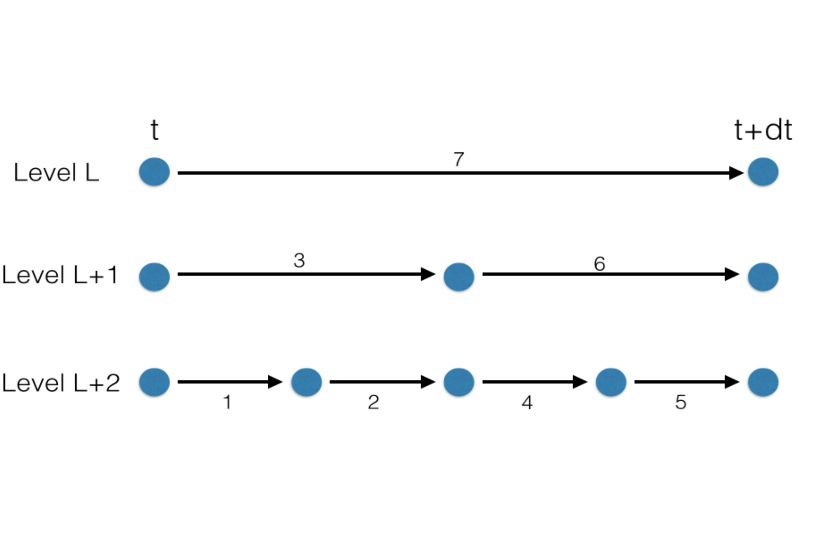
\includegraphics[width=.95\linewidth]{img/02/tstep.png}
\caption[Pas de temps AMR]{Gestion du pas de temps en fonction des niveaux raffinées.
Un niveau évolue par pas de temps deux fois plus court que celui de son niveau supérieur.
\label{fig:timestep}}
\end{figure}


\subsection{Gestion de l'expansion}
\label{sec:supercomobil}

%On parlera de simulations cosmologiques lorsque l'e volume considéré est en expansion.

%Nous avons vu dans l'introduction à la physique de la reionisation que l'énergie noire représente la majore partie du contenu de l'univers (cf \ref{sec:dark_egy}) .
%Nous allons voir dans cette partie comme cette composante est traitée numériquement.
%Bien que nous ne sachions absolument pas ce que peux être physiquement l'énergie noire, nous en observons les effets : l'Univers est en expansion accélérée.
%Le moteur gérant l'énergie noire n'est pas a proprement parler un moteur numérique, mais plutôt d'un système d'unité. % servant a normaliser la physique.
%Il consiste a normaliser les grandeurs par une variable fonction du facteur d'expansion.

L'intégration de la cosmologie, régissant le lien en le temps et le facteur d'expansion sera réalisé une fois au moment de l'initialisation du code (cf Eq. \ref{eq:scale_t}).
Il en résultera une table, conservée en mémoire pendant toute l'exécution.
Le facteur d'expansion sera alors interpolé dans cette table en fonction de l'avancement de la simulation.% (cf partie calcul du pas de temps) %TODO ref

Il existe deux possibilités pour modéliser l'expansion de l'univers à l'aide d'une grille.
La première consiste a considérer un élément de volume $dx$ de taille fixe, et au fur et a mesure que l'univers grandis, à y ajouter des éléments.
Le problème et que le coût numérique de la simulation croit, entre autre, avec le nombre d'éléments que l'on considère.
La seconde possibilité est de faire varier la taille des éléments de calcul avec le facteur d'expansion.
On appellera les longueurs ainsi exprimées des longueurs comobile.

\begin{equation}
r=a r'
\end{equation}

ou $r$ représente une longueur en unités physique et $r'$ en unités comobile.
Ainsi un cube de 10 Mpc physique de coté, pris aujourd'hui, aura une taille de 10 Mpc comobile (cMpc) aujourd'hui, mais aussi a redshift z=9 ou sa taille physique ne sera plus que de de 1Mpc physique.
De plus, il est généralement pratique de normaliser les grandeurs que l'on considère. 

\begin{equation}
r'=\tilde{r}r*
\end{equation}
ou $\tilde{r}$ est la longueur normalisée et $r*$ le facteur de normalisation.

La généralisation de ce principe a d'autre unités que la longueur est appeler système d'unités supercomobiles \citep{martel_convenient_1998}.

\begin{table}
\begin{center}
\begin{tabular}{r l} \hline 
Longueur: & $\tilde{r}=\frac{r}{ar_*}$ \\ \hline 
Densité de matière: & $\tilde{\rho}=\frac{\rho a^3}{\rho_*}$ \\ \hline 
Vitesse: & $ \tilde{v}=\frac{av}{v_*}$ \\ \hline 
Pas de temps: & $\tilde{dt}=\frac{dt}{a^2t_*}$\\ \hline 
Densité d’énergie potentielle: & $\tilde{\Phi}=\frac{a^2 \Phi}{\Phi_*}$\\ \hline 
Pression: & $\tilde{p}=\frac{a^5 p}{p_*}$\\ \hline 
Densité d’énergie cinétique: & $\tilde{\epsilon}=\frac{a^2 \epsilon}{\epsilon_*}$\\ \hline 
Densité D’éléments: & $\tilde{N}=a^3 N r_*^3$\\ \hline 
Flux: & $\tilde{F}=a^4 r_*^2 t_* F$\\ \hline 
\end{tabular} 
\end{center}
\caption[Système d'unité supercomobile]{Passage du système d'unités physique vers le système d'unités supercomobiles} 
\end{table}

\begin{table}
\begin{center}
\begin{tabular}{r l} \hline 
Longueur  & $r_*=L$\\ \hline 
Densité & $\rho_* = \bar{\rho} = \frac{3H_0^2 \Omega_m}{8\pi G}$\\ \hline 
Temps & $t_* = \frac{2}{H_0 \sqrt{\Omega_m}}$\\ \hline 
Vitesse & $v_* = \frac{r_*}{t_*}$\\ \hline 
Potentiel & $\Phi_* = \frac{r_*^2}{t_*^2} = v_*^2$\\ \hline 
Pression & $p_* = \frac{\rho_* r_*^2}{t_*^2} = \rho_* v_*^2$\\ \hline 
Énergie & $\epsilon_* = \frac{p_*}{\rho_*} = v_*^2$\\ \hline 
\end{tabular} 
\end{center}
\caption[Facteurs de normalisation]{Facteurs de normalisation des différents grandeurs physiques dans le système d'unités supercomobiles}
\end{table}

\subsubsection{Gestion du pas de temps}
L'évolution de la grille sera limité d'un pas de temps à l'autre.
La condition condition pour effectuer le calcul du pas de temps sera:
\begin{equation}
\frac{\delta a (\Delta t) } {a} < \epsilon
\end{equation}

\subsection{Recherche de voisin}
\label{sec:voisins}

Les processus physiques que l'on cherche a résoudre sont régit par des systèmes d'équations différentielles. (voir section \ref{sec:solvers})
En analyse numérique, une dérivée de $u$ suivant $x$ est localement approximée (dans le cas d'une différence finie centrée) par une équation de la forme :
\begin{equation}
\frac{d u}{dx} \approx \frac{u_{i+1}  + u_{i-1}}{2\Delta x}, 
\end{equation}
où $i$ est l'indice sur la grille de pas $\Delta x$.
Dans ce type de systèmes, l'état d'une cellule dépend donc des états des cellules qui l'entourent.

La recherche de voisins est une étape importante dans la gestion de la grille et se fera en suivant les étapes présenté sur la figure \ref{fig:voisin}.
Dans le cas ou la voisine se trouve dans le même OCT la recherche est immédiate.
Mais dans le cas ou la voisine n'est pas dans le même OCT, il faut trouver l'OCT voisin, vérifier que celui ci est géré par le même processus et vérifier si il est raffiné.
Cette recherche peut être complexe et couteuse, on prendra donc garde à minimiser les appels de la fonction de recherche. 

\begin{figure}
        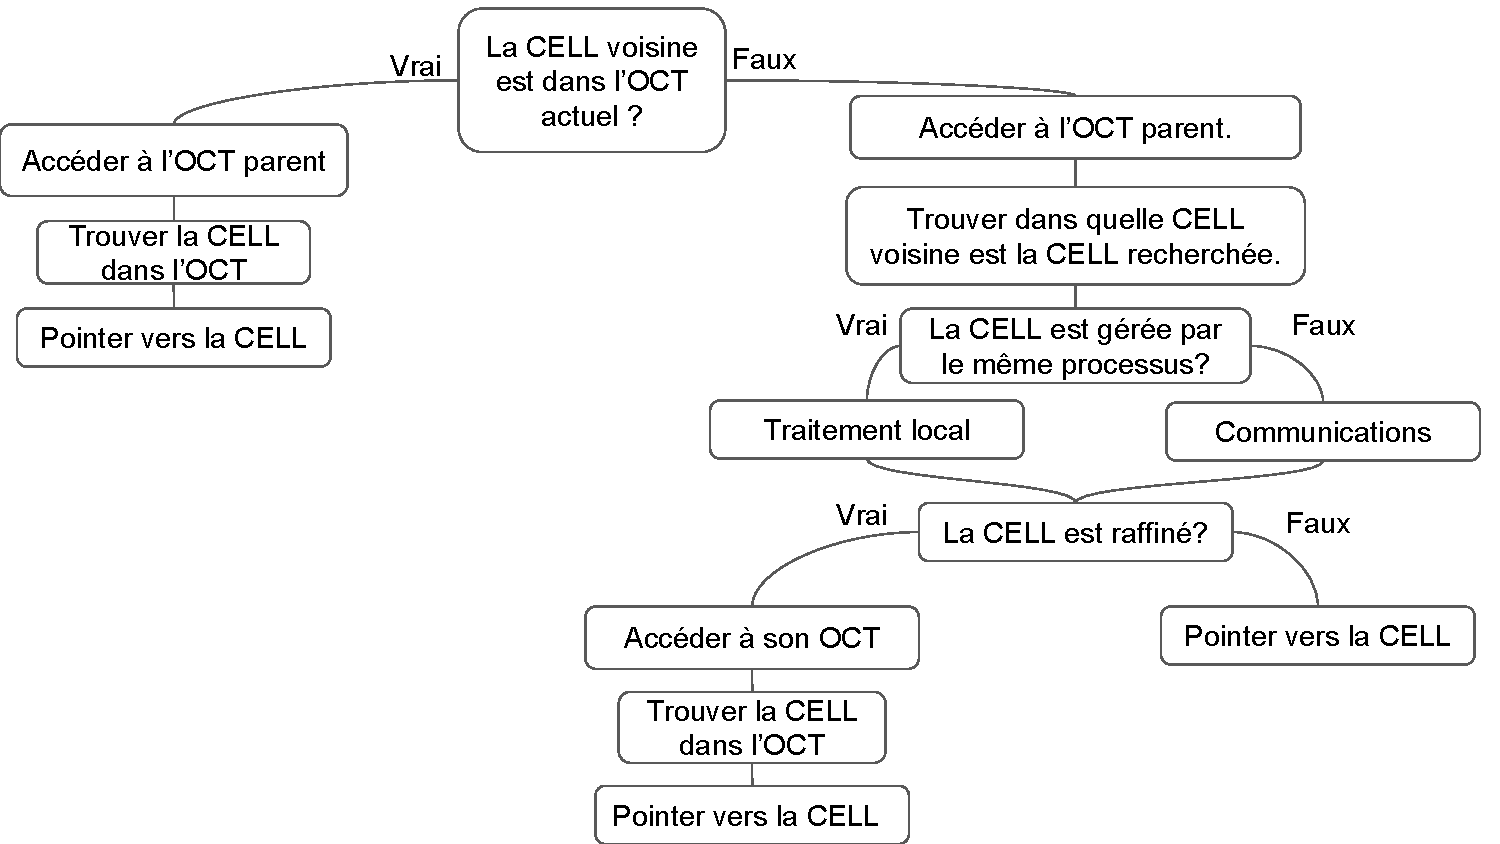
\includegraphics[width=\linewidth]{img/02/voisins.pdf} 
        \caption[Recherche de voisin dans l'octree.]{Arbre décisionnel pour la recherche de voisin dans l'octree.
        La recherche de voisins n'est pas triviale et peu avoir un coût non négligeable.
     	\label{fig:voisin} }
\end{figure}

%\begin{itemize}
%\item en fonction de l'ID de la cellule courante, déterminer si la voisine recherchée est dans le même OCT parent.
%
%\item
%\begin{itemize}
%\item Si c'est le cas: accéder à l'OCT parent, et à l'aide de l'indice du tableau de cellule, retrouver le voisin en question.
%\item Si ce n'est pas le cas, accéder à l'OCT parent, à l'aide des pointeurs sur les voisins, localiser l'OCT voisin et s'y rendre. Si l'OCT est raffiné déterminer 
%\end{itemize}
%
%\end{itemize}